\chapter{Telemanipulátor programja}
\label{sec:LatexTools}

Az telemanipulátor jelfeldolgozó rendszerének fizikai összeállítása után a szenzorok által küldött jelek szoftveres feldolgozását és használatát mutatom be. A fejezet során hasonlóan mint korábban a szenzoroktól kezdem a szoftveres komponensek bemutatását és haladok a tényleges robot mozgatásra szolgáló rendszerekig.

%----------------------------------------------------------------------------
\section{Szenzor kommunikációs protokollja}
%----------------------------------------------------------------------------
A GMR szenzor a mikrovezérlővel az úgy nevezett Synchronous Serial Communication \footnote{magyarul Szinkron Szériás Kommunikációs} röviden SSC protokolt használ. Ez a  protokoll egy olyan kommunikációs rendszer, amely során a küldő és a fogadó eszközök szorosan szinkronizáltak egymással a közös órajel alapján. Az SSC azon alapul, hogy mindkét eszköz előre rögzített órajelet használ a bekapcsolás pillanatától, hogy a rendszer használat teljes ideje alatt szinkronban maradjanak.

A protokoll közös órajele biztosítja, hogy a adat transzferálás esetén az órajel biztosítja, hogy mindkét eszköz azonos sebességgel és időzítéssel küldje és fogadja az üzenetet. Ez az információ küldés során bitek sorozataként továbbítódik, és a kommunikáló fogadó és küldő egységek egyeztetik az adatok kezdőpontját és végpontját az órajelet használva. Ennek következtében mindkét eszköz tudja, hogy mikortól kell és meddig értelmeznie az érkező biteket.

%TODO kép a GMR bitekről

A protokoll lehetővé teszi a teljes és a fél-duplex kommunikációt. Teljes-duplex esetén mindkét eszköz képes egyszerre küldeni és fogadni adatokat, míg fél-duplex esetén a kommunikáció váltakozva történik, azaz egyik eszköz küld, majd vált, és a másik eszköz fogad.

Az SSC gyakran használt alkalmazása az I2C (Inter-Integrated Circuit) és a SPI (Serial Peripheral Interface) kommunikációs protokollok. Az I2C esetén a kommunikáció két vezetéken, adatazon és órajelező vonalon történik, míg az SPI esetén több vezetéket használnak, például MISO (Master In Slave Out), MOSI (Master Out Slave In), órajeladóval és választóvonal.

A SSC protokoll széles körben alkalmazható az elektronikában és beágyazott rendszerekben, ahol szükség van a gyors, megbízható és szinkronizált adatkommunikációra a különböző eszközök között.

A telemanipulátor esetében half-duplex kommunikációs módot használok a GMR szenzor dokumentációjában meghatározott értéken (XYZ hivatkozás) állítottam be. Minden szenzorhoz tartozóan chipválasztó pineket is deklarálnom kellett. A kommunikációs protokoll kezeléséhez egy előre elkészített könyvtárat használtam, ami megtalálható a (XYZ melléklet) mellékletben.


\section{Mikrovezérlő program}
%----------------------------------------------------------------------------

A mikrovezérlő program a diploma dolgozathoz képest kisebb módosításokkal lett kiegészítve, de igazán nagy fejlesztést nem igényelt a program. A elvárásoknál támasztott elvárásoknak megfelelt. Kellően gyors és könnyen módosítható lett. (Fejezet hivatkozás XYZ)

A telemnanipulátornál használt program a konzulensem által készített hasonlóelven működő haptikus vezérlőjének(Hivatkozás XYZ) a mikrovezérlő programját vettem alapul. A programot gyorsan a saját eszközömhöz szükséges módosításokkal eltudtam látni, mivel ez az is STM32-es rendszerre lett készített.

Főkülönbségek, hogy a mikrovezérlő az én általam használt telemanipulátor esetében 7 szenzor adatait gyűjti össze, dolgozza fel és továbbítja a további rendszereknek.

A mikrovezérlő programba implementált funkciók a következők:

\begin{itemize}
\item Szögérték kiolvasás
\item Szögérték offszetelés
\item Szögérték Kinemtaikailag felvett forgás tengelyre igazítása
\item Szögértékek tömbértékek összegyűjtése
\item Kommunikáció a mikrovezérlőhöz csatlakoztatott számítógéppel
\end{itemize}

A szögértékeket szekvenciálisan az $1.$ csukló szenzortól a $7.$ csukló szenzorig egymásután olvassa ki. A szenzor kommunikáció már a bemutatott SSC kommunikáción történik és minden szenzor saját chipselect pin-jének a jelváltozására\footnote{A TLE 5012B GMR szenzor esetében alacsony jelről magas jelre vált a kommunikáció alatt} történik. A kiolvasott szögérték a szenzor meghatározott egyik tengelye és a mágnes kétpólusa által megadott póluspárok egymással bezárt szöge.

%TODO Kép a szenzor szögről.

Az a megkapott szögérték a $-180^\circ$ és $180^\circ$ közötti lehet. Ezt az értéket én át konvertáltam $0^\circ$ és $360^\circ$ fokos skálára ugyan is így sokkal könnyebben beállítható az offset és a forgás irány is egyértelműbb számomra. Az offszet paraméterek beállítása a program indulása után is változtatható, de alap paraméterek be vannak égetve. AZ oka ennek, így nem kellett minden tesztelési ciklus elején offszetelnem. A offszet értékeket a következő képpen állapítottam meg.

\begin{enumerate}
  \item Minden csuklón van egy jelző egyenes, ami a két tengely koordináta rendszereinek a párhuzamosságát jelenti abban az állásban
  \item A kinematikai felírásban vett koordináta rendszer szerinti nullába mozgattam a megfelelő csuklót
  \item Kiolvastam a szenzor adott pontú értékét
  \item Ha pozitív előjelű volt akkor kivontam, ha pedig negatív akkor hozzáadtam a kiolvasott értékhez az offszetet
\end{enumerate}

Az így megkapott szögértékek elfordulására kell még figyelni. Ugyanis a szenzor és mágnes elhelyezkedése a tengelyen befolyásolja, hogy a szögéréték a tengely körüli elfordulással melyik irányba pozitív. Ha a forgatási irány eltér egyszerűen a szögérték mínusz egyszeresét kell venni. 

Ezt követően, ha mindenszögértéket továbbítja a mikrovezérlő, ha igény van rá. Az igényt az interface támasztja a számítógépről még pedig, az UART porton küldött üzenettel. A jelenleg implementált parancsok:

\begin{itemize}
\item $RDS$ - Read from sensor - Szenzor értékek kiolvasás 
\item $KA$ - Keep Alive - Kapcsolat fenntartására vonatkozó parancs
\item $REC$ - Read Error Counter - Hibás kiolvasások darabszámának kiolvasása
\item $CEC$ - Clear Error Counter - Hibás kiolvasás számláló törlése
\end{itemize}

A fenti parancsok közül a REC, CEC és a RDS parancsokat használom. Az RDS esetén a szögértékek kiolvasásra kerülnek és továbbítódnak UART porton, ahogy korábban említettem. A továbbítás egy nagy méretű byte tömben történik, aminek az első két érték amit továbbít egy "OK" és maga az RDS paranccsal megkapott üzenet a többi érték a szenzorokból kiolvasott és számított szögértékek. A REC és a CEC parancsot a szenzorok üzembe helyezésekor használtam. Egy egyszerű port terminál kezelését lehetővé tévő programmal csatlakoztam a mikrovezérlőre és elküldtem a RDS parancsot kétszer. A két kiadott parancs között megváltoztattam a telemanipulátor orientációját. A beüzemelés alatt, több szenzor se működött azonnal és a CEC és REC parancsokkal tudtam a hiba darabszám tárolókat kiolvasni és törölni. A továbbiakban szeretnék még offszet érték beállítására vonatkozó metódust implementálni, illetve jelrögzítést és offszet-be állásra vonatkozó parancsokat.

A mikrovezérlő programmal kapcsolatban nagyon fontos még kitérni a RTOS (XYZ hivatkozás) rendszerre. Ez a STM32 vezérlőknél elérhető funkció a real-timehoz nagyon közeli működést tesz lehetővé. A program így előre megjósolható és determinisztikus módon válaszol az eseményekre, ugyanis realtime rendszerekben a feladatoknak szigorú időkorlátoknak kell megfelelniük, és az RTOS biztosítja a prioritáskezelést, időosztást és egyéb funkciókat a hatékony valós idejű működés érdekében.

%TODO rtos kép

A kritériumokban(XYZ) meghatározott $4[ms]$ vagy gyorsabb lefutás a robot vezérlés eléréséhez nagyban hozzájárul ez a lehetőség. A RTOS-sel elérhető párhuzamos lefutószerű működés és a szigorúan definiált feladatok a mikrovezérlő szögérték kiolvasási feladatát biztosítja, hogy megfelel a kritériumoknak.

\subsection{UART port}
%----------------------------------------------------------------------------
Az "UART" rövidítés a "Universal Asynchronous Receiver/Transmitter" kifejezést takarja. Az UART egy soros kommunikációs protokoll, amely a digitális adatok átvitelét teszi lehetővé két eszköz között. Ez a protokoll olyan eszközök közötti soros kommunikációt biztosít, amelyek között nincs központi órajel (asynchronous), tehát az adatküldés és -fogadás időzítése a két eszköz között előre nem megállapodott.

Az UART általában két vezetéken keresztül történik: TX (Transmitter) és RX (Receiver). Az adatok a TX vezetéken keresztül mennek egyik eszköztől a másikig, és a RX vezetéken keresztül az ellenkező irányban. A kommunikációt start és stop bitek, valamint adatbitek alkotják.

A UART port vagy interfész tehát a hardver vagy a vezérlő, amely lehetővé teszi az UART protokollt támogató eszközök közötti kommunikációt. Az UART portok széles körben alkalmazottak például számítógépek, mikrovezérlők, beágyazott rendszerek és egyéb eszközök kapcsolódási pontjaiként. Az UART segítségével a különböző eszközök adatokat küldhetnek és fogadhatnak egymástól, amely lehetővé teszi a sokféle elektronikai eszköz közötti egyszerű és megbízható kommunikációt.

\section{Haptikus interfész}
%----------------------------------------------------------------------------

A mikrovezérlő a számítógéphez, amin ez az interface fut UART porton(XYZ fejezet) csatlakozik. A telemanipulátor csuklóiban mért szenzor jeleket a haptikus interface kéri el a mikrovezérlőtől. A haptikus jelző ebben az esetben azt jelenti, hogy visszajelzés is van építve a rendszerbe. A sikeres megfogás vagy ütközés esetén a haptikus interface képes a openmanipulátor (XYZ melléklet) vezérlő telemnanipulátorába épített rezgő motoroknak jelet adni. Az általam készített telemanipulátorba nincs ilyen típusú visszajelzés beépítve. Az interface ezt a visszajelzési visszacsatolást leszámítva tökéletesen megfelel az általam kitűzött célnak. Ezt a szoftveres megoldást annak ellenére, hogy nem egy az egyben a saját munkám fontosnak tartom bemutatni, hogy a tovább fejlesztési lehetőségeknél kitudjak arra térni, hogy miért lenne fontos ezt az eszköz interfacet tovább módosítani és fejleszteni.

Az interface két részre bontható. Az első az, ami megvalósítja a kommunikációt a mikrovezérlővel a másik pedig egy ROS node, ami a telemanipulátorból kiolvasott szögjeleket publikálja. Az szerial kommunikáció egy egyszerű "USB"-s csatlakozásnak minősül, ami azt jelenti, hogy lehetőség van információt küldeni és kiolvasni a port-ról. A csatlakoztatott mikorvezérlő a fizikai porton jelenik meg a számítógép port listájában Linuxon ez a $tty*$ portok között van. Fontos megjegyezni, hogy a teljes dolgozatom Ubuntu vagy közimsertebb nevén Linux operációs rendszeren lett megvalósítva. Windows operációs rendszeren is van lehetőség futtatni, ebben az esetben viszont virtuális gépet\footnote{Olyan programok amelyek képesek Windows operációs rendszeren telepített programban valamilyen nem Windows környezetre készített programot futtatni} vagy Windows Subsystem for Linux\footnote{Microsoft által támogatott virtuális Linux operációs rendszer. A egyik legelterjedtebb megoldás arra, hogy Windows operációs rendszerrel rendelkező eszközökön Linux-ot futassunk} - rövidítve WSL - kell használni. Természetesen számos más megoldás van, mint például a dual-Boot\footnote{Linux és Windows operációs rendszerek ugyanazon eszközön egymás mellé a háttértárba fel vannak telepítve és a számítógép elindulásánál lehet megválasztani, hogy melyiket akarjuk indítani. Ebben az esetben sokkal kiegyensúlyozotabb hardver terhelést kapunk és teljes értékű operációs rendszerekkel dolgozunk, ami a stabilitást nagy mértékben javítja.}. Én a diploma dolgozatomban bemutatott telemanipulátor esetében teljesértű Linux operációs rendszerrel ellátott illetve dual-Bootos számítógépet használtam.

A fizikai szerial kommunikáció létrejötte utána az interfacenek ugyanazok a kommunikációs paraméterek lettek beállítva, mint amit a mikorvezérlő is használ. Ez triviális ugyanis, ahogy a XYZ fejezetben bemutattam a UART prtokolt fontos, hogy a két eszköz szinkronban legyen. A beállított paraméterek:

\begin{itemize}
\item Baudrate (Kommunikáció sebessége) - $115200 [-]$
\item Paritás Bit (Hibajelző bit) - Nincs
\item Stop bit szám - $1 [db]$
\item Byte méret - $8[db]$
\end{itemize}

Ezzel létrejött a programban is használható kommunikációs kapcsolat a számítógép és a mikrovezérlő között. Az interface ezt követően ciklikusan $8[ms]$-onként a kommunikációs porton az RDS parancs segítségével lekérdezi a csuklószögeket. A visszakapott választ ellenőrzi, hogy az előző fejezetben bemutatott sorrendben minden rendben megérkezik-e és így validálva az adatok helyességét. A megkapott csukló szögeket átváltja radiánba és a ROS topológián (XYZ melléklet ros top) is láthatóan publikálja őket.

\subsection{ROS}
%----------------------------------------------------------------------------
A Robot Operating System, röviden ROS, egy nyílt forráskódú, rugalmas és elosztott szoftverrendszer, amelyet a robotok fejlesztéséhez és irányításához használnak. Az alábbiakban összefoglalom a ROS rendszert, kitérve a node-okra, a topic-okra és a robotrendszerekben történő alkalmazásukra.

A ROS egy gráfalapú rendszer, amelyben a különböző komponenseket, úgynevezett node-okat, összekapcsolják egymással, hogy információt és parancsokat cseréljenek. A node-ok önálló folyamatok, amelyek futnak és kommunikálnak egymással. Minden node specifikus feladatokat lát el, például szenzoradatok gyűjtése, adatfeldolgozás, irányítás vagy más műveletek végzése.

A node-ok közötti kommunikáció a topic-okon keresztül történik. A topic egy adatcsatorna, amely lehetővé teszi a node-ok közötti aszinkron adatátvitelt. Egy node publikálhat adatokat egy topic-ra, és más node-ok feliratkozhatnak erre a topic-ra, hogy megkapják az adatokat. Ez a központi kommunikációs mechanizmus a ROS rendszerben. Például egy szenzor node adatokat publikálhat egy "lidar" nevű topic-ra, és egy navigációs node feliratkozhat erre a topic-ra, hogy megkapja a szenzoradatokat és használhassa őket a robot navigációjához.

A ROS rendszer különösen népszerű a robotrendszerek fejlesztésében és irányításában. A robotok általában több szenzorral rendelkeznek, amelyek adatokat gyűjtenek a környezetről, például távolság, helyzet, kép vagy hanginformációk. Ezeket a szenzoradatokat a ROS node-ok gyűjtik és feldolgozzák. Emellett a robotoknak vezérlési parancsokat kell fogadniuk és végrehajtaniuk. A ROS lehetővé teszi a vezérlő node-ok létrehozását, amelyek az irányítást végzik, például a robot mozgását vagy más műveleteit vezérlik.

A ROS rendszerben a node-ok és topic-ok rugalmasan konfigurálhatók és összekapcsolhatók, ami lehetővé teszi a fejlesztők számára a moduláris és újrafelhasználható szoftverkomponensek létrehozását a robotalkalmazásokhoz. Ez a moduláris szerkezet elősegíti a fejlesztés hatékonyságát, és lehetővé teszi a különböző csapatok számára, hogy párhuzamosan dolgozhassanak az egyes részegységeken.

Összességében a ROS egy erőteljes és rugalmas szoftverrendszer, amely lehetővé teszi a fejlesztők számára a robotrendszerek fejlesztését és irányítását. A node-ok és topic-ok használata lehetővé teszi az adatok gyűjtését, feldolgozását és megosztását a rendszer komponensei között, ezáltal segítve a robotok működését és irányítását különböző feladatok végrehajtása során.

\section{Universal Robot kontroller}
%----------------------------------------------------------------------------

A csukló szögekkel már elegendő információ van ahhoz, hogy megállapítsuk a telemanipulátor által felvett pillanatnyi TCP pontot. Ez a pont a telemanipulátor 0. koordináta rendszerének és az end effektorának távolsága és orientációja. Ez a egydimenziós tömb ami magába foglal hat paramétert, amelyek $x,y,z$ koordináta és $\alpha,\beta,\gamma$ orientációs szögeket tartalmazza. Az elméleti háttérről a XYZ. fejezetben részletesen kitértem.

A TCP pontok pontos értékét a telemanipulátorra elkészített DH transzformációs mátrixxal tudom megadni. A paraméterek számítása folyamatosan az új csuklószög értékekkel folyamatosan történik. A program, ami ezt a számítást végzi nevezem a robot kontrollernek. Ennek a feladata az, hogy a telemanipulátorok szögértéke alapján meghatározza a TCP pontot és továbbítsa a robot felé, akár szimulációs környezetben, akár valós robot meghajtásáról van szó.

A robot kontroller másik feladata a munkatér mozgatása. Indítása előtt meg lehet neki adni $[x,y,z] [mm]$ mátrixban, hogy a valós koordináta pontokat mennyivel és milyen irányba tolja el. Ezzel a lehetőséggel minden típusú robottal lehet használni, illetve a munka területet folyamatosan lehet válzotatni a robot számára, amihez idomítani lehet. Az orientációs paramétereket nem lehet befolyásolni.

A kontroller fel van készítve biztonsági funkciók ellátására is. Objektumok formájában definiálni testeket a térben, amelyek kimetszhetnek területet a telemanipulátor és a elmozgatás által meghatározott munka területből.

A fenti műveletek elvégzése utána a kontroller pozíció és orientációs paramétereket átadja egy $MoveGroupInterface$ objektumnak, ami a jelenlegi megoldás szerint kapcsolatot teremt a robot vezérlő rendszere és a kontroller között. Ez az objektum quaternion paraméter lista szerint dolgozza fel az adatokat, ami miatt az általam megadott hat darab paramétert át kell konvertálni ebben az értelmezésbe.

A $MoveGroupInterface$ a kapott cél paraméterek és a robot jelenlegi pozíciója alapján, amit a következő szegmenstől kap kikalkulálja a robot következő orientációját, amivel megtudja valósítani a kívánt TCP pontot. Itt már megjegyezés kell tennem, hogy a legnagyobb gondot a robot vezérlésnél az okozza, hogy a telemanipulátor által felvett TCP pont és a megvalósítható robot orientációk megadás nagyon számítás igényes.

\subsection{Robot mozgás pályatervezők}
%----------------------------------------------------------------------------

A diploma dolgozatom leadása pillanatában hasznát kontroller mellett számos más lehetőség is van arra, hogy a robotot a cél orientációba vezéreljük. Erre azért fontos kitérni, mert a valós robot mozgatásnál látható lesz, hogy a korábbi ROS verzió és az abban használt MoveIt kontroller nem a leggyorsabb pályatervezést eredményezi annak ellenére, hogy a hardver képes lenne nagyobb teljesítménnyel is működtetni a robotot. Annek érdekében, hogy személetesebb legyen az, hogy miért fontos ezeknek a rendszereknek a számítási kapacitácával foglalkozni rövid listában összefoglaltam mi a logikai sorrendje a robot vezérlőknek:

\begin{enumerate}
\item Célállapotot vagy trajektória meghatározása, amit a robotnak követnie kell
\item Lekérdezi a robot aktuális orientációját, csukló szögeit
\item Meghatározza a jelenlegi állapot és a cél állapot közti eltérést
\item A különbség alapján vezérlő jelet ad ki a robotvezérlőnek
\item Változás bekövetkezett-e és ha igen akkor a ciklus kezdődik elölről
\end{enumerate}

A legfontosabb arra kitérni, hogy mivel a diplomám célja nem a tökéletes kontroller létrehozása volt így egy általános megoldást használok jelenleg, ami a mindenre jó így igazán semmire elven nem a legoptimálisabb kontroller. Sokkal specifikusabb a telemanipulátor karakterisztikájára és a cél hardver tulajdonságaira optimalizált kontrollert is létre lehet hozni a MoveIt-tal, viszont ez a prototípus tervezésének ebben a szakaszában még nem prioritás.

Egy másik aspektusból vizsgálva a MoveIt azon verziója, ami jelenleg hajtja a robotot program nyelv verzió szerint is régebbi megoldásokkal lett elkészítve. Ez egyenesen vezet ahhoz az eredményhez, hogy programozói nyelven szólva bottleneck \footnote{A "bottleneck" kifejezés olyan helyzetet vagy pontot jelent, ahol a rendszer vagy folyamat teljesítménye egy vagy több korlátozó tényező miatt korlátozott. Ez a korlátozó tényező olyan, mint egy szűk nyakú palack, ami lassítja vagy akadályozza a folyamatot vagy rendszert, és megakadályozza, hogy az az elvárt teljesítményt nyújtsa.}-kel, azaz a rendszer más elemei képesek lennének nagyobb teljesítményt elérni, de valamilyen program technikai megoldás miatt ez nem lehetséges.

A fent leírt problémákra a ROS és a MoveIt fejlesztői is kínálnak már megoldást, ezek a megoldások ráadásul még a valós idejű működést is biztosíthatják. A ROS 2 önmagában több valós idejű támogatást kínál a kiterjesztett hardver interface illetve a dinamikus változás/változó kezelés, ami robot tekintetében kulcsfontosságú. Ez hasznosságát úgy lehet szemléltetni, hogy egy robot esetében a a pálya tervezés az egy folyamtatos idő kritikus metódus, ha valós időben szeretnénk vezérelni. A tervezés így szinkron metódusként lehet kezelni.

%TODO Ez egy kicsit még vérszegény

Konkrét megoldásként lehet a MoveIt2 servo kontrollere, ami pontosan a valósidejű robot vezérlésre lett kifejlesztve. Ez a kontroller differenciál kinematikai alapelven működik és teheti lehetővé a valósidejű vezérlést. Ez azt jelenti, hogy a kontollernek ugyan úgy cél koordinátákat és orientációs szögeket adunk meg viszont a robot vezérlő nem a pozíciót adja tovább a robotnak, hanem azt hogy a robot csuklóinak milyen sebességen és meddig kell működnie. Ez a számítási módszer megoldás lehet a telemanipulátoros vezérlésre is, de a diploma leadása pillanatában még, csak a Moveit servo alkalmazhatóságát ismerkedtem.

\subsection{Quaternion}
%----------------------------------------------------------------------------
A quaternion egy speciális típusú matematikai objektum, amely gyakran használatos térbeli orientációk és rotációk reprezentálására, például robotika, grafika, és számítógépes játékok területén. Egy négydimenziós számsorozat, és a következőképpen írhatók le:

\begin{equation}
a + b \textbf{i} + c \textbf{j} + d \textbf{k} 
\end{equation}

ahol az $a$ skalár rész, $b$,$c$,$d$ pedig a vektori rész koordinátái, és $i$,$j$,$k$ a komplex egységvektorok, amelyek kielégítik a következőt: 

A quaternionok előnye, hogy hatékonyan reprezentálhatnak rotációkat a háromdimenziós térben, és nem szenvednek a "gimbal lock" nevű problémától, amely bizonyos Euler-szögparamétereknél jelentkezik.

\begin{figure}[!ht]
\centering
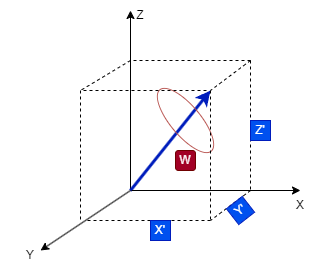
\includegraphics[width=70mm, keepaspectratio]{figures/Diagrammok/Quaterion}
\caption{Quaterion térvektor által megvalósítható rotáció szemléltetése}
\label{fig:Quaterion}
\end{figure}

Ezzel a módszerrel történő rotációk gyakran alkalmazhatók például térbeli orientációk számítására a robotika vagy számítógépes grafika területén. A rotációkat általában egy kezdeti orientáció és egy célorientáció közötti kvaternióként reprezentálják, majd ezeket a kvaterniókat alkalmazzák a térbeli objektumokon.

Fontos megjegyezni, hogy a quaternionok bevezetése és használata egy speciális terület a matematikában, és gyakran igényel némi megértést a térgeometriában és lineáris algebrában.


\section{Gazebo szimuláció}
%----------------------------------------------------------------------------

A célkitűzésem egyik az volt, hogy a telemanipulátorral szimulációs környezetben tudjak vezérelni egy robot kart. ezt azért tartom nagyon fontos lépcsőfoknak a valós robot vezérlést megelőzően, mert kvázi előellenőrzése az elkészített rendszernek. Bármilyen súlyos matematikai hiba vagy súlyos anomália, ami veszélyeztetné a robot épségét szimulációnál jelentkezni fog. A szimulációt Gazebo-val készítettem és teszteltem. Ugyanazt a hardvert használtam amin később a valós robot vezérlést is végeztem, így sikerült meggyőztem arról hogy a hardver és a szoftveres rendszer is megfelelően működik. A szimulációs robot vezérlés sikerült és egy Universal Robot 5-ös típusú robot az elvárásoknak megfelelően sikerült vezérelni szimulációs környezetben.

A szimulációs rendszerek alapvető tulajdonsága, hogy az szimulálják le, ami fel van nekik programozva. Ezeket a szimulációs elemeket a teljesség igénye mellett se lehet egy az egyeben megfeleltetni a valós megfelelőjüknek és ebből fakadólag előfordulhatnak pálya tervezési hibák, zajok és olyan előre nem lekezelt program futásbeli hibák, amik a programok rossz időbeli sorrendje miatt keletkeznek. Ezeket a problémákat jellemzően a szimulációs rendszer korlátjainak tekintjük. Az általam futtatott szimulációnál, csak azokra a tapasztalatokra térek ki, amik közvetlenül a telemanipulátor, a kontroller és a robot vezérlő működésével kapcsolatos. Tapasztalatokat összegzem és a valós robot vezérlésénél össze is fogom hasonlítani.

%TODO Kép a szimulációról

Egy meghatározott cél koordináta és a jelenlegi között nincs nagy távolság akkor gyorsan végrehajtja a parancsot. Nagy távolság esetén a számítási idő szignifikánsan nagyobb. Ez akár egyértelmű is lehet viszont egy nagyon nagy hátrány, mert nem is feltétlen a TCP pontok távolsága számít hanem az az egyenlet rendszer, aminek eredménye ként a lehetséges orientációkat megkapjuk. Ezzel kapcsolatosan megfigyeltem még, hogy a nagyon összetett pályák esetén még a $5[s]$-os időtúlépést is elérheti kontroller, amikor is a számítás kiáll hibára és megszakítja a kalkulációt. Ezt követően vagy visszatér és egy következő orientációt kezd el számolni, vagy helytelen orientáció miatt beavatkozást igényel. Amit még a valós robot szimulációval való korrekt összehasonlítás miatt fontos volt megfigyelnem, hogy stabil egy adott pontban, nem érzékelhető se remegés se bizonytalan pozíciótartás.

A szimulációs tesztelés sikeres volt. Ez a megközelítés a későbbiekben is hasznos lehet, ha új funkciók vagy modul cseretörténik a rendszerben. Így mindent nagy vonalakban lelehet tesztelni mielőtt valós roboton elindítanánk.


\section{Valósrobot vezérlése}
%----------------------------------------------------------------------------

A diploma dolgozatom végcélja az volt, hogy egy valós robotot is vezéreljek a telemanipulátorommal. 

A robot, amit valójában sikerült mozgatnom, ugyan az a robot amit a szimulációs környezetben is teszteltem. A robotot laboratóriumi összeállításban teszteltem ezért is látszik, hogy egy sakk tábla van a robot előtt és nem egy témába vágó műtő fatnom, mert a laboratóriumi körülmények között mások kollégák is használták. A laboratóriumban a szimuláció és a valós vezérlés közti alapvető különbségekre voltam kíváncsi.

%TODO Kép a robot

Az egyértelműen kijelenthető, hogy sikerült a robotot vezérelni és közel azonos tapasztalatokat gyűjtöttem, mint a szimuláció esetében. A tervezési idő erősen függ a kezdő és végpont távolságától, illetve ugyanúgy időtúllépéssel le áll mint a szimuláció esetében. Lényeges különbség viszont, hogy nagyon látványos megjelenik egy nyugvó pont körüli zaj. A robot kismértékben remeg/mozog olyankor amikor a telemanipulátor által a vezérlő nem ad direktben mozgás utasítást. Ez nagyon nagy gond, mivel a sebészeti szimulációk vagy későbbiekben műtő fantom operálására szeretném tovább fejleszteni, akkor ez mozgás megengedhetetlen, de ezt a következő fejezetben részletesebben bemutatom.

A valós robot mozgatással sikeresnek tekintettem a fejlesztésnek ezt a szakaszát. Az elképzelésemet meglehet valósítani, ennek a pontosítását már további munkával lehet javítani. 

\section{Koncepcionális hibák}

Az előző fejezetben a robot mozgatásnál tapasztalt mozgásnak és remegésnek több oka lehet, amelyek közül néhány ismert a számomra.

A mikrovezérlőtől indulva a szenzorok jele a feldolgozás során a gyártó által jelezve is $1^\circ$-os hibával működhet. Például ha ez az első csuklóban jelenik meg példa kedvéért pozitív irányban, akkor a end-effektor $x$ vagy $y$ irányban közel $6[mm]$ is lehet, ami elfogadatlan. Egyértelműen ilyen nagy mértékű hiba az nagyon szélsőséges esetben jelenhet meg. Viszont kisebb szöghibák a hat csuklón halmozottan okozhatnak bármelyik tengelyen hasonló nagyságrendű hibát. A szöghiba zajszűrésére lehetőség van, de nagyon körül tekintően kell csinálni, mivel a GMR szenzorok előnye pont abban van, hogy érzékenyek a kis mágneses tér változásra. A legegyszerűbb, de nem a legolcsóbb lehetőség, ha redundánsan csuklónkként egy pár szenzor párt használok ezzel akár átlagolás, akár felülbírálói megoldással tudom csökkenteni a hibát.

A zajnak a másik oka szintén ebből a szöghibából adódik, de a kontrollerben nem elnyomódik, hanem felerősödik. Ennek nem fizikai, hanem matematikai oka van ugyanis a kinematikai számítások összetettsége, miatt kerekítés a számítások során. A kerekítések nem feltétlen a számítási kapacitás hiánya, hanem a vezérelni kívánt robot ismétlési pontossága miatt is lehetséges. A UR 5 ismétlési pontossága a gyár adatok alapján $0,1[mm]$ és $0,03[mm]$ között lehet. Azt, hogy a remegés emiatt lenne érezhető s robotkarban kevésbé tartom valószínűnek. Arra, hogy a remegés mi miatt jön létre a robotban mindenképpen szeretnék választ találni.